%\iffalse
\let\negmedspace\undefined
\let\negthickspace\undefined
\documentclass[journal,12pt,twocolumn]{IEEEtran}
\usepackage{cite}
\usepackage{circuitikz}
\usepackage{amsmath,amssymb,amsfonts,amsthm}
\usepackage{algorithmic}
\usepackage{graphicx}
\usepackage{textcomp}
\usepackage{xcolor}
\usepackage{txfonts}
\usepackage{listings}
\usepackage{enumitem}
\usepackage{mathtools}
\usepackage{gensymb}
\usepackage{comment}
\usepackage[breaklinks=true]{hyperref}
\usepackage{tkz-euclide} 
\usepackage{listings}
\usepackage{gvv}                                        
\def\inputGnumericTable{}                                 
\usepackage[latin1]{inputenc}                                
\usepackage{color}                                            
\newtheorem{theorem}{Theorem}[section]
\usepackage{array}                                            
\usepackage{longtable}                                       
\usepackage{calc}                                             
\usepackage{multirow}                                         
\usepackage{hhline}                                           
\usepackage{ifthen}                                           
\usepackage{lscape}
\newtheorem{problem}{Problem}
\newtheorem{proposition}{Proposition}[section]
\newtheorem{lemma}{Lemma}[section]
\newtheorem{corollary}[theorem]{Corollary}
\newtheorem{example}{Example}[section]
\newtheorem{definition}[problem]{Definition}
\newcommand{\BEQA}{\begin{eqnarray}}
\newcommand{\EEQA}{\end{eqnarray}}
\newcommand{\define}{\stackrel{\triangle}{=}}
\theoremstyle{remark}
\newtheorem{rem}{Remark}
\begin{document}
\bibliographystyle{IEEEtran}
\vspace{3cm}
\title{GATE 21 EE/29}
\author{EE23BTECH11040 - Manoj Kumar Ambatipudi$^{*}$% <-this % stops a space
}
\maketitle
\newpage
\bigskip
\renewcommand{\thefigure}{\theenumi}
\renewcommand{\thetable}{\theenumi}
\textbf{QUESTION:}
In the circuit, switch 'S' is in the closed position for a very long time. If the switch is opened at time $t=0$, then $i_L\brak{t}$ in amperes, for $t\geq0$ is
\begin{figure}[h]
    \renewcommand\thefigure{1}
    \centering
    \begin{circuitikz}[american]
    \draw (0,0) to (1,0) to (1,-2) to [R=$4\Omega$] (3,-2) to [V=$30V$,invert] (5,-2) to (5,0) to  [R=$1\Omega$] (7,0) to [L=$0.5H$] (7,-4) to (0,-4) to [V=$10V$,invert] (0,0);
    % Draw the open switch
    \draw (1,0) to[ospst] (5,0);
    % Add a label for the open switch
    \node at (3,0.8) {\scriptsize{Open at $t=0$}};
    % Draw the arrow and label for current
    \draw [->] (6.6,-1.4) -- (6.6,-2.7);
    \node at (6.4,-1.9) {$i_{L}$};
    \end{circuitikz}
    \caption{Circuit in $T$ domain}
    \label{fig:EE_21_29_1}
\end{figure}
\\
\textbf{Solution:}
%\fi
\begin{table}[h]
\renewcommand\thetable{1}
    \centering
    \begin{tabular}{|c|c|c|}
    \hline
         Variables&Description&value  \\\hline
            $i_L\brak{0}$   &    Initial current in Inductor & 10A\\\hline
            L     & Inductance of Inductor & 0.5H\\\hline
    \end{tabular}
    \caption{Caption}
    \label{tab:EE_21_29_1}
\end{table}

Circuit in $S$ domain is
\begin{figure}[h]
\renewcommand\thefigure{2}
    \centering
    \begin{circuitikz}[american]
    \draw (0,0) to [generic=$R_1$] (6,0) to [generic=$R_2$] (8,0) to (8,-3) to [generic=$R_4$] (6,-3) to [generic=$R_3$](2,-3) to [generic=$sL_3$] (0,-3) to (0,0) ;
    \draw (5,0) to  (5,-1);
    \draw (5,-2) to (5,-3);
    \draw (5,-1.5) circle [radius=0.5];
    \node at (3.7,-1.5){Detector};
    \draw (0,-1.5) to [short, *-] (-0.5,-1.5) to (-0.5,-4.5) to [sV, l_=$V_{\text{AC}}\brak{s}$] (8.5,-4.5) to (8.5,-1.5) to [short, -*] (8,-1.5);
    \draw (5.3,0) to (5.3,1) to [generic=$\frac{1}{sC_2}$](8,1) to (8,0);
    \end{circuitikz}
    \caption{Circuit in $S$ domain}
\end{figure}
\\
From \figref{fig:EE_21_29_1}, $i_L\brak{0}$ can be found using steady state analysis. Writing $KVL$ , we get
\begin{align}
    10-i_L\brak{0} &= 0\\
    i_L\brak{0} &= 10\label{eq:EE_21_29_1}
\end{align}
Writing $KVL$ for \figref{fig:EE_21_29_2},
\begin{align}
    \frac{10}{s} - I_L\brak{s}\brak{4+1+0.5s} + \frac{30}{s} + Li_L\brak{0} &= 0\\
    \implies I_L\brak{s} &= \frac{sLi_L\brak{0}+40}{5s + 0.5s^2} 
\end{align}
From \tabref{tab:EE_21_29_1}, 
\begin{align}
    I_L\brak{s} &= \frac{2.5s+40}{5s + 0.5s^2}\\
    I_L\brak{s} &= \frac{10s+80}{10s + s^2}\\
                &= \frac{8}{s} + \frac{2}{s+10}
\end{align}
Taking Inverse Laplace, 
\begin{align}
    i_L\brak{t} &= \brak{8+2e^{-10t}}u\brak{t}
\end{align}
\begin{figure}[h]
\renewcommand\thefigure{3}
    \centering
    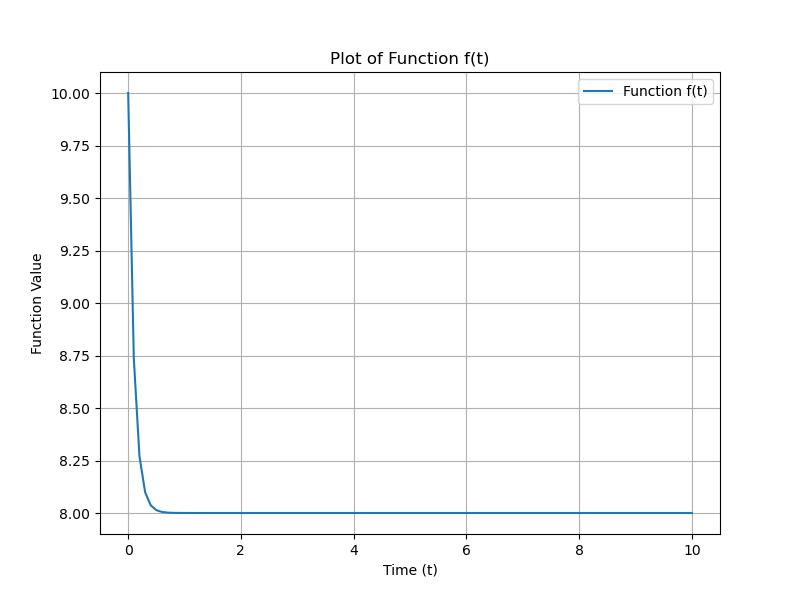
\includegraphics[width=1.0\columnwidth]{figs/fig_3.jpg}
    \caption{Plot of $i_L\brak{t}$ taken from Python3}
    \label{fig:EE_21_29_1}
\end{figure}
\end{document}
